\documentclass[12pt]{article}
\usepackage[english]{babel}
\usepackage[utf8x]{inputenc}
\usepackage[T1]{fontenc}
\usepackage{listings}
\usepackage{tikz}
\usepackage{/Users/songye03/Desktop/math_tex/style/quiver}
\usepackage{/Users/songye03/Desktop/math_tex/style/scribe}

\begin{document}
Songyu Ye

These are notes from my meeting with Tara on March 11.

\section{Introduction}
I asked about the $T$-equivariant cohomology of $S^4$. There is a lot to consider.
Recall that $S^4$ corresponds to two copies of $\C\P^2$ "glued along a copy" of $\C\P^1$.
This corresponds on the level of moment polytopes of the following picture:

\begin{center}
	\includegraphics[scale = .1]{/Users/songye03/Desktop/math_tex/img/tara1.jpeg}
\end{center}
In this picture I have two bases written down. One basis corresponding to the GKM story
is the one given by Morse theory. The other basis, corresponding to the multiplicative basis
$x_1,x_2,x_3$ comes from looking at Chern classes of line bundles on the facets.

\hfill

In particular on $\C^d$ ($d$ being the number of facets) there is a trivial line bundle
$\C_i\times \C^d \to \C^d$ and this descends to a line bundle on the symplectic reduction $\C\P^{d-1}$.

\hfill

In the case of $\C\P^2$ we have three line bundles and their Chern classes correspond to the
multiplicative basis depicted. To convert between them and the localization story, we can
see that localizing these Chern classes at a fixed point is the outward pointing edge vector
(the class is only supported on the facet).
\begin{center}
	\includegraphics[scale = .1]{/Users/songye03/Desktop/math_tex/img/tara2.jpeg}
\end{center}
In the case of $S^4$ the moment graph is no longer embedded in space but we can still make sense of
divisibility conditions. In particular, the moment graph for $S^4$ corresponds to
(see the drawing) the divisbility conditions $t_1t_2 \mid f_2 - f_1$.

\hfill

The hope is that we can write down some presentation for the equivariant cohomology of toric origami
manifolds similar to the following presentation for toric varieties \begin{align*}
	H_T^*(M) = \frac{\C[x_1,\ldots,x_n]}{I}
\end{align*} one generator for each facet and the ideal $I$ generated by the facets whose
intersection is empty. Note that if one believes that the classes are only supported on the vertices corresponding
to the facet, then of course products of facets which do not intersect will be zero. The suprising
part is that these are all the relations.

\hfill

\red{We hope that for toric origami manifolds we can write down a similar presentation. The first step is
	perhaps going from the Morse theory basis to the multiplicative basis in the $S^4$ case.}
\begin{center}
	\includegraphics[scale = .1]{/Users/songye03/Desktop/math_tex/img/tara3.jpeg}
\end{center}


\subsection{ABBV Formula}
In this sectino we began by considering the Euler class of the null foliation.


Consider the ABBV formula which expresses the pushforward of an equivariant class in terms
of the restriction of the class to the components of the fixed point set.

\hfill

Let $A$ index the components of the fixed point set and let $\alpha \in H_T^*(M)$. Integration
along $M$ is defined as the pushforward of the map $M\to p$. Then the ABBV formula states that
\begin{align*}
	\int_M \alpha = \sum_{a\in A} \frac{\int_{M_a}\alpha\vert_{M_a}}{e_a}
\end{align*} where $e_\alpha$ is the equivariant normal
class of the normal bundle to $M_a$.

\hfill

Tara says that we can use this formula to compute self-intersection numbers
in the 4-manifold setting. In particular let's look at the
polytope for the Hirzebruch surface

\begin{center}
	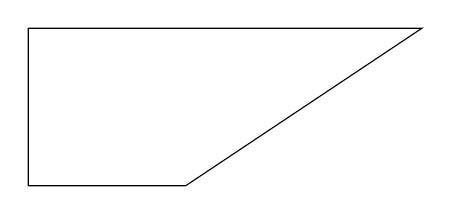
\begin{tikzpicture}
		\draw (0,0) -- (2,0) -- (5,2) -- (0,2) -- cycle;
	\end{tikzpicture}
\end{center}

Consider the class $\alpha$corresponding to the bottom facet. The relevant ABBV computation says that \begin{align*}
	\int_M \alpha^2 = \frac{\int_{M_1}\alpha^2\vert_{M_1}}{e_1} + \frac{\int_{M_2}\alpha^2\vert_{M_2}}{e_2}
\end{align*} we consider $\alpha^2$ because we are thinking about
the self-intersection of the class $\alpha$. The class $\alpha$ is supported on the bottom facet.
The numerator corresponds to look at the restriction of $\alpha^2$ to that particular fixed point.
The denominator looks at all outward pointing edge vectors of the fixed point.
Thus we get that \begin{align*}
	-k = \frac{y^2}{xy} + \frac{(y+kx)^2}{-x(y+kx)}
\end{align*} which is indeed true.

\red{Multiply this picture by a trivial bundle and think about what the right computation is
	in the 3 dimensional case.}

\section{References}
\begin{itemize}
	\item https://msp.org/agt/2015/15-4/p14.xhtml
	\item https://www.sciencedirect.com/science/article/pii/S0926224599000273?via%3Dihub
\end{itemize}
Come back and tell Tara about the her paper with Ana.

\end{document}